% ================
% Landon Buell
% 
% 
% 26 May 2020
% ================

\documentclass[12pt,letterpaper]{article}

\usepackage{amsmath,amssymb,amsfonts}
\usepackage{algorithmic}
\usepackage{graphicx}
\usepackage{textcomp}
\usepackage{xcolor}
\usepackage{subfigure}
\usepackage{pgf}
\usepackage{multirow}

\usepackage[left=2.5cm,right=2.5cm,top=2.5cm]{geometry}

\begin{document}


\textcolor{red}{Place for Landon}

\subsection{Case Study 1: Multilayer Perceptron}

\paragraph*{}The purpose of this case study was to develop an understanding for how the multilayer perceptron (MLP) neural network architecture is affected by a \textit{bit muting} attack function. This type of attack would seek to manipulate the values of a floating-point number at a binary level. In the case of this experiment, we have chosen to model a function that forces the most-significant-bit (MSB) in the exponent of floating-point number to be muted to $0$. In each MLP model, numerical values were stored as double precision floating-point numbers as per the IEEE 754 standard.

%\paragraph*{}Of the $64$ bits in the double precision float, $11$ are dedicated the the exponent, the 1st of which is the MSB. By asserting this bit be zero, the exponent is can only be composed of $10$ dynamic bits, that subtracting the exponential offset of $1023$ gives a maximim base-10 value of $0$. To save computation time, rather than convert a a float directly to binary string and mute the MSB, the command \textit{numpy.frexp(z)} was used to break apart a float $z$ into it's mantissa, $M$, and exponent $E$ such that $z = M \times 2^E$. If the value of $E$ is ever above, $0$, it is then set to $0$, otherwise it is left unmodified. Note that the value was set to $0$, rather than subtract $1023$ to save further computation time and avoid invalid ranges when converting the mantissa and exponent back into it's floating-point counterpart.

\paragraph*{}After a a single floating-point number has it's MSB muted, it is then constrained to lie on the open interval $(-1,+1)$. A map of input values against MSB output values is shown in fig. (\ref{MUTE MSB}). The inputs are a subset of the possible values of a double precision floating-point numbers for visual ease.

\begin{figure}[h]
\label{MUTE MSB}
\begin{center}
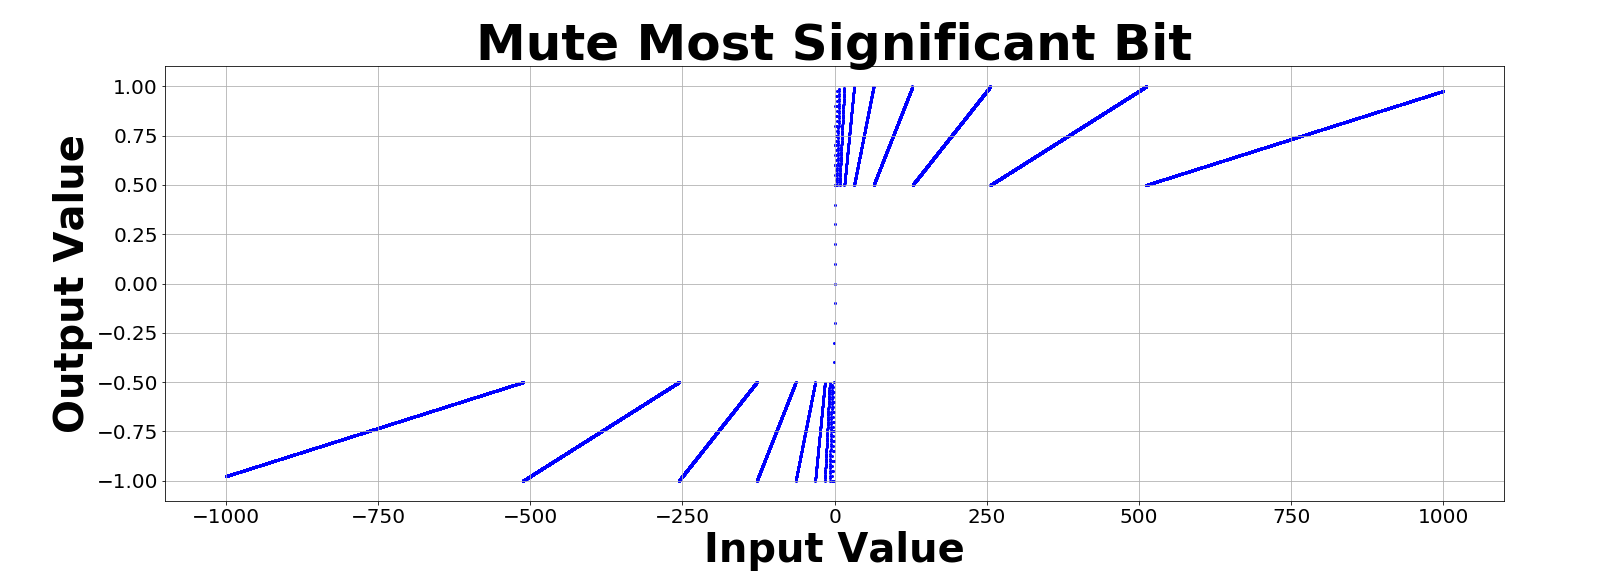
\includegraphics[scale=0.3]{Mute_Most_Significant_Bit}
\end{center}
\end{figure}

\paragraph*{}


\subsubsection{Experimental Setup}
CNN model, layers, neurons, forward backward propagation
what data set you used 
describe the attack function

\paragraph*{}The MLP neural network model is composed of multiple layers of \textit{neurons}, that each contain a real-valued floating-point number called an \textit{activation}. Layers of neurons interact with the neurons in adjacent layers in sequence though a series of weighting coefficients, and bias elements, which is then subjected to an activation function. In general, given a layer of activations $\vec{x}^{(l)}$ (The superscript is used as a layer index), the activations in the next sequential layer, $\vec{x}^{(l+1)}$, are produced with weighting matrix $\hat{W}^{(l)}$, bias vector $\vec{b}^{(l)}$, and activation function $f$ such that:

\begin{equation}
\label{feed-forward}
\vec{x}^{(l+1)} = f \Big( \hat{W}^{(l)} \vec{x}^{(l)} + \vec{b}^{(l)} \Big)
\end{equation}

The recurrence of equation (\ref{feed-forward}) is used to pass information forward through the network. In a network with $L$ layers, raw information is given with $\vec{x}^{(0)}$ and the network's prediction is given by the final layer, $\vec{x}^{(L-1)}$.

\paragraph*{}The Multilayer Perceptron network must then find a series of parameters, which are the elements in all weighting matrices and all bias vectors, that allows for a given sample to produce a low value for a given \textit{Loss function}. The loss function measures the difference between a networks given output and expected output; with better trained networks producing generally low loss values over a set of samples. The process of finding the values is called \textit{optimization}. There are many different algorithms that perform optimization, and for this experiment, we have chosen to use \textit{Stochastic Gradient Descent} (SGD) due to its widespread use and versatility.

\paragraph*{}To model a bit-muting attack, we introduce and \textit{attack function} that acts in the matrix-vector product 
$\hat{W}^{(l)} \vec{x}^{(l)}$ in eqn. (\ref{feed-forward}). When a Boolean \textit{trigger condition} parameter is met, the MSB attack as described above, eqn. (\ref{feed-forward}) is instead replaced with it's attack variant:

\begin{equation}
\label{Attack}
\vec{x}^{(l+1)} = f \Big( A \big[ \hat{W}^{(l)} \vec{x}^{(l)} \big] + \vec{b}^{(l)} \Big)
\end{equation}

Where $A$ is the attack function, applied element-wise to each object in it's argument. Equation (\ref{Attack}) is then producing a perturbation from expected values that is not explicitly acounted for in the optimization procedure.

\subsubsection{Impact of muting attack on four metrics}

To measure the impact of this type of attack on the image classifier model, we test a baseline classifier against one subset to the 

add picture before and after attack


add pictures (results) and draw conclusion










\end{document}